\section{Architectural Overview: Basic TC System}

The \tcs system includes three main components: The \tcontract, the \encname, and the \medname.

The \tcontract (denoted more concisely by \tcont) is a smart contract that acts as the blockchain front-end of the \tc service, and thus an interface between relying contracts and \tc. It accepts datagram requests from requesters and returns corresponding datagrams from \tc. Additionally, the \tcontract manages \tc monetary resources, both fees and gas (in Ethereum). 

The \encname and \medname reside on the \tc server. The \encname runs in an enclave, an SGX-protected execution environment in the server. As enclaves lack network access, the \medname handles bidirectional network traffic on behalf of the \encname, providing network connectivity to the blockchain (the Ethereum system) and to data sources queried by \encname. Additionally, \medname acts as a web server handling off-chain service requests from clients. The \medname is an ordinary user-space application. It does not benefit from special hardware protection and thus, unlike the \encname, can be subverted by an adversarial OS on the \tc server, causing network delays or failures.

The \encname ingests and fulfills datagram requests. To obtain the data composing datagrams, it queries external data sources, specifically HTTPS-enabled internet services. To obtain and keep track of the state of datagram requests, it monitors the state of \tcontract on the blockchain; thus \tcontract forwards datagram requests implicitly to the \tc server. (In the initial version of \tcontract, the \encname's view of the blockchain also comes from a data source.) Additionally, the \encname may be queried by a client to provide supplies off-chain, hardware-backed \emph{attestations} on the state of the \encname---both its executing code and its clock. It is to support this service that \medname includes a web server.

Briefly, then, the end-to-end processing of a datagram request is initiated by a requester \reqcont sending a datagram request to \tcont on the blockchain. (For example, the request may specify in \dgform the value of the DJIA index at time $t$ = the close of market on 15 Jan 2016.) Using network services provided by the \medname, the \encname obtains the request from the blockchain. It contacts a data source (e.g., https://www.google.com/finance) to obtain the requested data at time $t$, and composes a datagram $\dgm$, which it sends back to \reqcont.

\begin{figure}[t]
\centering
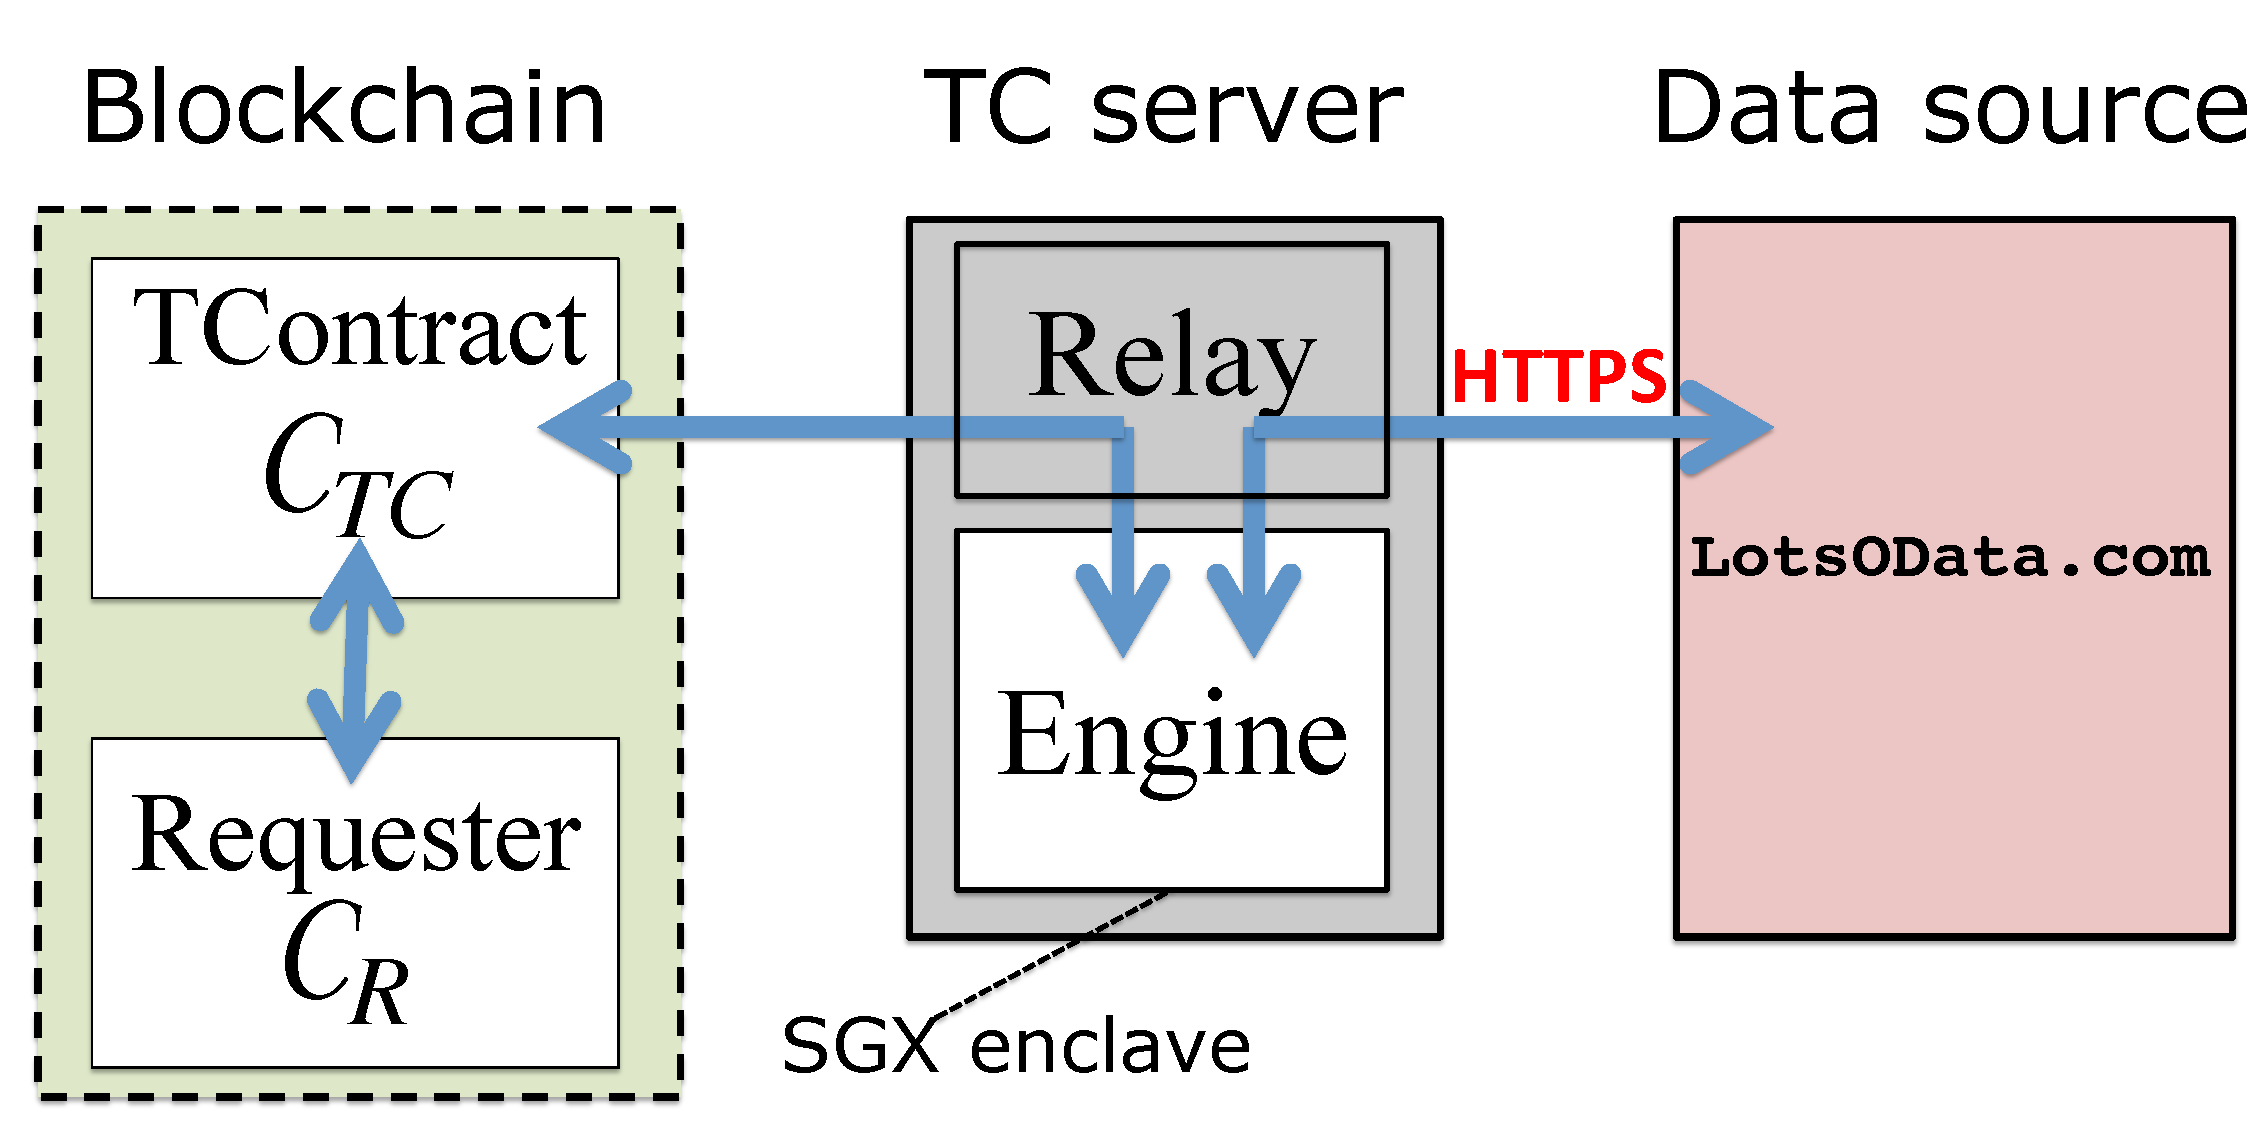
\includegraphics[width=\columnwidth]{OverviewFig}
\caption{{\bf Basic Town Crier architecture.}}
\label{fig:schematic}
\end{figure}

We now explain in detail the data flow around a datagram request. 

\subsection{Data flow and notation}


We denote a datagram instance by $\dg$. It includes the complete (digitally signed) message $\dgreq$ from the requester to a \tc contract $\tcont$ on the blockchain; $\dgreq$ includes both a specification $\dgform$ of the requested datagram and a payment $\dgpay$, which includes (in Ethereum) gas to cover the cost of the request as well as a fee. Finally, $\tcont$ receives a return message $\dgret$ from the $\tc$ service. As contracts cannot send messages, \tc makes use of an address $\tcadd$ on the blockchain to transmit this message to $\tcont$. Then $\tcont$ returns the associated data $\dgm$ to $\reqcont$. 



\subsection{Client API}
\subsection{TC server}
\subsubsection{Trusted executable}
\subsubsection{Untrusted executable}
\subsection{TC Blockchain resources}
These include the TC contract and the addresses from which it sends messages and manages its wallet
\subsection{Security model}


